\section{DetectAnyLLM Framework}
DetectAnyLLM builds upon Fast-DetectGPT~\cite{fastdetectgpt}, which determines whether a text is MGT by measuring the log-probability discrepancy between the original text and its perturbed variants~\cite{detectgpt}.
%
This method involves three key steps: \textit{1) re-sampling the given text}, \textit{2) computing the discrepancy between original text and re-sampled text}, and \textit{3) making a decision using the discrepancy}.
%
In \Cref{3.1}, we describe how the log-probability discrepancy is calculated.
%
Next, in \Cref{3.2}, we explain the motivation behind our improvements to this detection process, along with the specific designs we introduce.
%
Finally, in \Cref{3.3}, we detail how discrepancy is ultimately used for MGTD within our proposed framework.

\subsection{Preliminary}\label{3.1}


\noindent \textbf{Basic Hypothesis. }
%Our work shares a same hypothesis with ~\cite{fastdetectgpt} and ~\cite{detectgpt}, that is, 
Machine-generated text tends to consist of high-probability tokens at each position, whereas human-written text has greater variability.
%
Although sampling strategies like top-k and top-p introduce some randomness, LLMs still generally select tokens with relatively high probabilities.
%
Thus, features in the probability distribution of tokens can serve as useful cues for distinguishing machine-generated text from human-written.


\noindent \textbf{Probability Discrepancy. }
Given a text $x$ and a scoring model $f_\theta$, when using another language model $q_\phi$ to produce perturbations, the \textit{probability discrepancy} (i.e., probability curvature)~\cite{detectgpt} can be expressed as:
\begin{equation}
    d(x, f_\theta, q_\phi) = \log f_\theta(x) - \mathbb E_{\tilde{x} \sim q_\phi(\cdot|x)}[\log f_\theta(\tilde{x})],
    \label{3.1.1}
\end{equation}
where $\tilde{x}$ is the perturbed version of $x$ by $q_\phi$.

% Based on the hypothesis, machine-generated text $x_m$ tends to have high log-probability, whereas its perturbed version $\tilde{x_m}$ shows a lower log-probability.
% %
% In contrast, human-written text $x_h$ generally has a lower log-probability.
% %
% When perturbed, $\tilde{x_h}$ tends to show an increase in log-probability, as the perturbation process replaces words in $x_h$ with higher-likelihood alternatives according to the model.
% %
% Thus, we expect to achieve:
% \begin{equation}
%     d(x_m, f_\theta, q_\phi) > d(x_h, f_\theta, q_\phi).
%     %\tag{3.1.2}
%     \label{3.1.2}
% \end{equation}
% %
% This inequality forms the basis of MGTD~\cite{detectgpt, fastdetectgpt, imbd}.

% When calculating this discrepancy, achieving $f_\theta$ is straightforward, allowing $\log f_\theta(x)$ to be efficiently computed using a Markov chain.
% %
% However, estimating the expectation of the log-probability of $\tilde{x}$ is more complex.
% %
% DetectGPT~\cite{detectgpt} addresses the estimation by generating many perturbations $\tilde{x}$ and approximating the expectation using the mean log-probability of these samples.
% %
% Since log-probabilities are computed using a Markov chain, even a small perturbation requires recalculating the entire chain, thus DetectGPT~\cite{detectgpt} has a high computational complexity.
% While effective, this approach requires computing log-probabilities for numerous perturbations, making it computationally expensive and less practical for real-world applications.

When calculating this discrepancy, achieving $f_\theta$ is straightforward, allowing $\log f_\theta(x)$ to be efficiently computed.
%
However, since the log-probabilities are computed using Markov-Chain, even a small perturbation requires recalculating the entire chain.
%
Thus, estimating the expectation of the log-probability of $\tilde{x}$ is complex.

\noindent \textbf{Fast-DetectGPT. }~\cite{fastdetectgpt} introduced \textit{conditional probability}, which provides a biased yet computationally efficient estimation of the original probability:
\begin{equation}
    f_\theta(\tilde{x}) = \prod_{i}f_\theta(\tilde{x}_i|\tilde{x}_{<i}) \sim \prod_{i}f_\theta(\tilde{x}_i|x_{<i}) = f_\theta(\tilde{x}|x).
    %\tag{3.1.3}
    \label{3.1.3}
\end{equation}
%
By introducing Eq.~\eqref{3.1.3}, the probability discrepancy in Eq.~\eqref{3.1.1} can be further reformulated to the\textit{conditional probability discrepancy}:
\begin{equation}
    d_c(x, f_\theta, q_\phi) = \frac{\log f_\theta(x|x) - \tilde{\mu}}{\tilde{\sigma}},
    %\tag{3.1.4}
    \label{3.1.4}
\end{equation}
where
\begin{equation}
\begin{aligned}
    \tilde{\mu} &= \mathbb E_{\tilde{x}\sim q_\phi(\tilde{x}|x)}[\log f_\theta (\tilde{x}|x)],\\
    \tilde{\sigma}^2 &= \mathbb E_{\tilde{x}\sim q_\phi(\tilde{x}|x)}[\log f_\theta (\tilde{x}|x) - \tilde{\mu}^2].
\end{aligned}
%\tag{3.1.5}
\label{3.1.5}
\end{equation}
% In Eq.~\eqref{3.1.4},  $\log f_\theta(x|x)$ is a unbiased estimation of $\log f_\theta(x)$, which is the first item of Eq.~\eqref{3.1.1}.
% %
% In addition,  $\tilde{\mu}$ is a biased estimation of $\mathbb E_{\tilde{x}\sim q_\phi(\cdot|x)}[\log f_\theta(\tilde{x})]$, representing the second term in Eq.~\eqref{3.1.1}.
%
Noticing that a normalization item $\tilde{\sigma}$ is added into the discrepancy function, we further explore how the $\tilde{\sigma}$ affects performance in ~\Cref{ablation_on_sigma}.
%
% This normalization enhances detection accuracy and ensures that discrepancy distributions remain comparable across different models and datasets, thus improves robustness in real-world applications.
%
Eq.~\eqref{3.1.4} forms the discrepancy we use in our study.

Based on the hypothesis, machine-generated text $x_m$ tends to have a high log-probability, whereas its perturbed version $\tilde{x_m}$ shows a lower log-probability.
%
In contrast, human-written text $x_h$ generally has a lower log-probability.
%
When perturbed, $\tilde{x_h}$ tends to show an increase in log-probability, as the perturbation process replaces words in $x_h$ with higher-likelihood alternatives according to the model.
%
Thus, we expect to achieve:
\begin{equation}
    d(x_m, f_\theta, q_\phi) > d(x_h, f_\theta, q_\phi).
    %\tag{3.1.2}
    \label{3.1.2}
\end{equation}
%
This inequality forms the basis of MGTD~\cite{detectgpt, fastdetectgpt, imbd}.

% Observing Eq.~\eqref{3.1.4}, we note that that  the discrepancy $d$ increases when $f_\theta$ assigns a higher probability to $x$ than to its perturbed version $\tilde{x}$.
% %
% Based on our \lichongyi{our?} hypothesis, since the scoring model $f_\theta$ prefers high-probability tokens at each position, detection performance can be improved by increasing the probability discrepancy between MGT and HWT within the model’s output distribution.
% %
% To achieve this, \cite{imbd} introduced \textit{Direct Preference Optimization (DPO)}~\cite{dpo} and believed that utilizing DPO to optimize instead of using MSE, enables the model to learn stylistic features more effectively, thereby enhancing the robustness of the detector.
% %
% However, we suggest that DPO can only help the scoring model learn to be another LLM rather than a detector. This creates a gap in the model’s ability to handle MGTD effectively
% \lichongyi{preliminary is overlength. Some content can be removed to Introduction. Moreover, we cannot copy the content from the original paper. In Preliminary, just present the basic idea and workflow, even the limitations.}

\begin{figure}[t]
    \centering
    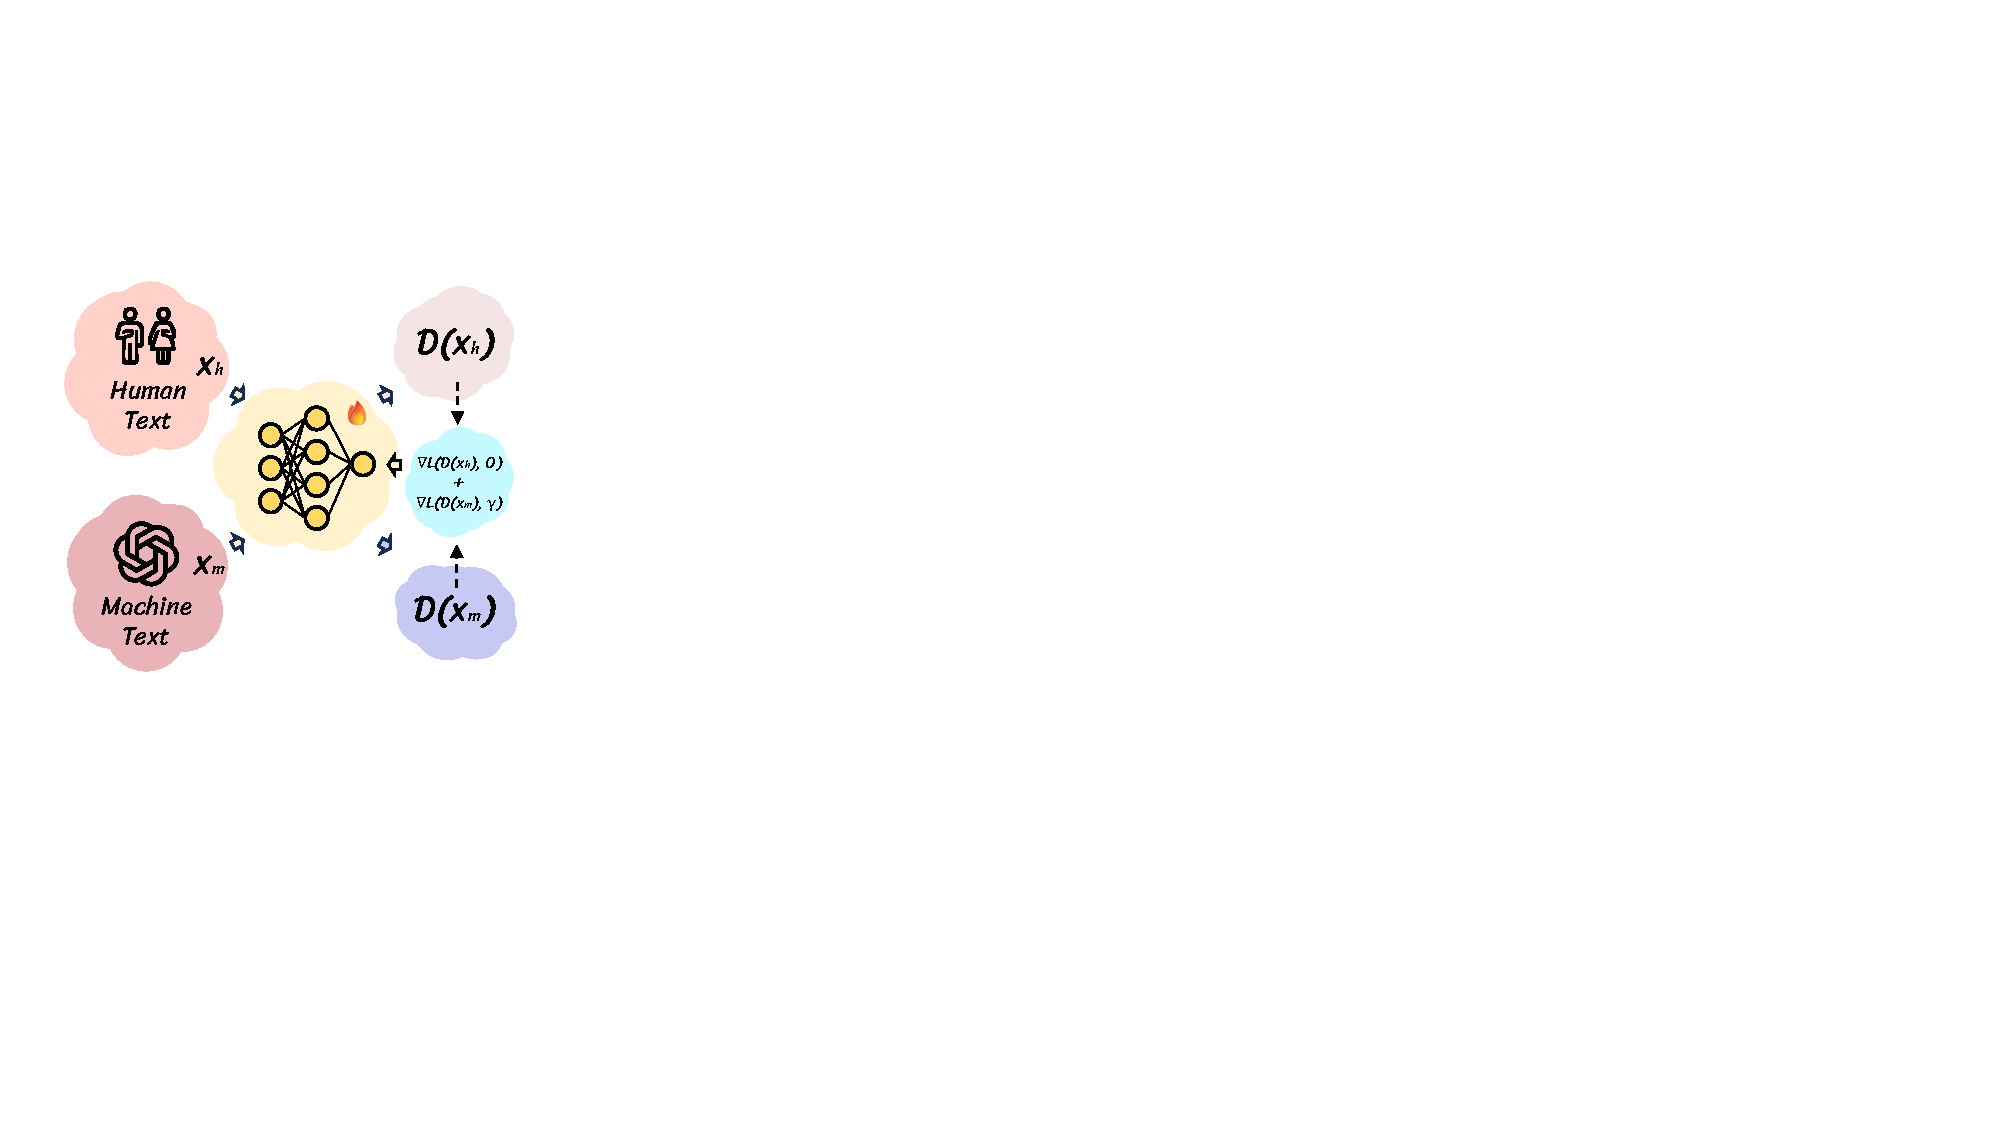
\includegraphics[width=0.65\linewidth]{fig/ddl.pdf}
    \caption{Overview of Direct Discrepancy Learning. The scoring model receives paired HWT-MGT data and computes the discrepancy for each. We optimize it to minimize the HWT's discrepancy while maximizing the MGT's.}
    \Description{Overview of Direct Discrepancy Learning. }
    \label{fig:ddl}
\end{figure}

\subsection{Optimizing by Direct Discrepancy Learning}\label{3.2}
As shown in Eq.~\eqref{3.1.4} and Eq.~\eqref{3.1.2}, the key to enhance the detector's performance is to increase the scoring model's probability distribution discrepancy between MGT and HWT.

While ImBD~\cite{imbd} has achieved significant performance gains by incorporating \textit{Direct Preference Optimization (DPO)}~\cite{dpo} to optimize the scoring model, we argue that DPO is not the optimal optimization method for the MGTD task.
%
This is because DPO implicitly aligns the scoring model with the preferences of another language model, rather than directly optimizing the scoring model to classify MGT and HWT. 
%
Moreover, such alignment could mislead the scoring model from learning the MGTD-oriented knowledge, thus do harm to the detector's generalization performance.


\noindent \textbf{DPO.}
~\cite{dpo} is derived from the optimization objective of \textit{Proximal Policy Optimization (PPO)}~\cite{ppo}, which is:
\begin{equation}
    \mathop{max}_\theta \mathbb{E}_{x\sim f_\theta(x)}[r(x)] - \beta\mathbb{D}_{KL}[f_\theta(x) \mid \mid f_{ref}(x)],
    \label{3.2.1}
\end{equation}
where $x$ is a text sampled from the scoring model $f_\theta$'s distribution, and $r$ is a reward function that can judge whether this sample is bad or good.
%
By analyzing and re-parameterizing this optimization objective, we can obtain DPO's optimization objective:
\begin{equation}
    \mathop{max}_\theta \mathbb{E}_{x_m, x_h \sim \mathop{D}}[\log \sigma(\beta\log\frac{f_\theta(x_m)}{f_{ref}(x_m)}-\beta\log\frac{f_\theta(x_h)}{f_{ref}(x_h)})],
    \label{3.2.6}
\end{equation}
where $x_m$ denotes MGT and $x_h$ stands for HWT.
%
$f_{ref}$ is a reference model, usually the original $f_\theta$.
%
The detailed derivation process will be presented in the supplementary material.

\noindent \textbf{Redundant KL-regularization. }\label{redundant KL-regularization}
The KL-regularization between $f_\theta$ and $f_{ref}$ is explicitly added to the optimization objective in PPO~\cite{ppo}, and its weight is adjusted via $\beta$, as shown in Eq. \eqref{3.2.1}.
%
While in DPO~\cite{dpo}, as Eq. 
\eqref{3.2.6} shown, such regularization is implicitly embedded in the optimization objective, and its strength can also be adjusted by $\beta$.
%
ImBD~\cite{imbd} directly adopts Eq.\eqref{3.2.6} as its loss function and leverages paired MGT-HWT data to optimize the scoring model $f_\theta$.
%
The KL-regularization forces the scoring model to retain its internal knowledge while learning preferences.

\textit{This leads us to question: for the MGTD task, what is the significance of retaining the original knowledge of the scoring model during training?}

Since we have already collected data and introduced training, our direct objective should be enable the scoring model to better learn the features of the source model from the training data.
%
While fundamentally, we hope that the training process will teach the scoring model how to become a detector.
%
However, the KL-regularization drastically shifts this objective: from learning the intrinsic knowledge of the MGTD task to aligning the scoring model with the distribution of training data.
%
Thus shifts the training process from learn a detector to learn a language model.
%
Such an optimization objective fails to directly reflect task requirements, thereby limiting the detector's performance potential.

%Experiments on the impact of the KL-strength $\beta$ on ImBD~\cite{imbd} is provided in the Supplementary Material.

\noindent \textbf{Direct Discrepancy Learning. }
We observed that by simply removing the KL-regularization from the optimization objective, the robustness and generalization of the model can be significantly improved. Thus, the optimization goal can be re-written as:
\begin{equation}
    \mathop{max}_{\theta} \mathbb{E}_{x\sim \mathop{D}}[r(x)].
    %\tag{3.3.1}
    \label{3.3.1}
\end{equation}
Furthermore, we utilize a simple reward function $r(x)$, defined as:
\begin{equation}
    r(x) = \begin{cases}
    -\Vert \gamma - d_c(x, f_\theta, q_\phi) \Vert_1, & \text{when $x$ is $x_m$,}\\
    -\Vert d_c(x, f_\theta, q_\phi) \Vert_1, & \text{when $x$ is $x_h$.}
    \end{cases}
    %\tag{3.3.2}
    \label{3.3.2}
\end{equation}
where $\gamma$ is an hyper-parameter.
%
This reward function is designed based on the conclusions discussed in Section~\ref{3.1}, that is the discrepancy of human-written text $x_h$ tends to be low (close to 0) while the discrepancy of machine-generated text $x_m$ tends to be positive.
%
The parameter $\gamma$ is introduced to control how positive the discrepancy of $x_m$ should be.
%
In our experiment, $\gamma$ is arbitrarily chosen.
%
As ~\Cref{tab:ablation_gamma}, experiment on the impact of the value of $\gamma$, shown that the model's performance is not particularly sensitive to this choice, indicating a level of robustness to variations in $\gamma$. 
%
In practice, our input consists of paired HWT-MGT data. We set $q_\phi = f_\theta$ following the ImBD~\cite{imbd}'s setting, which allows us to use the scoring model’s output for optimization: 
\begin{equation}
    \mathop{min}_\theta \mathbb{E}_{x_m, x_h \sim \mathop{D}}(\Vert d_c(x_h, f_\theta, f_\theta)\Vert_1 + \Vert \gamma - d_c(x_m, f_\theta, f_\theta)\Vert_1).
   % \tag{3.3.3}
    \label{3.3.3}
\end{equation}
We call this optimization method as \textit{Direct Discrepancy Learning (DDL)}, as it helps the scoring model directly learning the discrepancy between MGT and HWT.

%\noindent \textbf{Analysis. }
By removing the KL-regularization, the scoring model can essentially forget its identity as a language model and instead focus on learning task-oriented knowledge, which is critical for the MGTD task.
%
Furthermore, we introduce a reward function based on the discrepancy $d_c$, which incorporates a task-oriented prior, and thus can further help the scoring model learn the knowledge of MGTD.
%
Specifically, $d_c$ for HWT approaches $0$, while $d_c$ for MGT is positive.


\subsection{Detecting by Reference Clustering}\label{3.3}
We use \textit{Reference Clustering} to achieve the transition from $d_c(x)$ to $p_{m}(x)$.
%
Specifically, this algorithm is designed to estimate the probability of a given value belonging to a specific distribution, consisting of: \textit{data aggregation} and \textit{probability estimation}.

\noindent \textbf{Data Aggregation. }
We first collect a certain number of MGT texts as the MGT reference dataset $M$, and an approximately equal number of HWT texts as the HWT reference dataset $H$.
%
Then, we employ the scoring model $f_\theta$, which will be used for detection, to respectively compute the conditional probability discrepancy $d_c$ for each text in $M$ and $H$.
%
Thereby , we can obtain the conditional probability discrepancy distribution $D_m$ and $D_h$ of the texts in $M$ and $H$ under scored by $f_\theta$.


\noindent \textbf{Probability Estimation. }
We select the value in $M\cup H$ that is $k_{th}$ closest to the target value $d_c(x)$ as the search window $\delta$:
\begin{equation}
    \delta = sorted(\{\Vert d_c(x_{ref}) - d_c(x)\Vert_1 \mid x_{ref}\in M \cup H\})[k],
    \label{3.3.4}
\end{equation}
where $k$ is a hyper-parameter that should be determined by the size of reference dataset.
%
For a larger reference dataset, a larger $k$ is better as it can provide higher precision of $p_{m}(x)$.

Then, we count the number of MGT texts and HWT texts within the window range:
\begin{equation}
    \begin{aligned}
        cnt_m = \sum_{d\in D_m}I(d_c(x) - \delta < d < d_c(x) + \delta),\\
        cnt_h = \sum_{d\in D_h}I(d_c(x) - \delta < d < d_c(x) + \delta).
    \end{aligned}
    \label{3.3.5}
\end{equation}
Finally, we estimate the probability that text $x$ belongs to MGT using the local statistical ratio:
\begin{equation}
    p_m(x) = \frac{cnt_m}{cnt_m + cnt_h}.
    \label{3.3.6}
\end{equation}

Since the window $\delta$ is adaptively determined by the data distribution, this method can maintain stability under different data densities, thereby improving the robustness of real-world MGTD.

\begin{figure*}
    \centering
    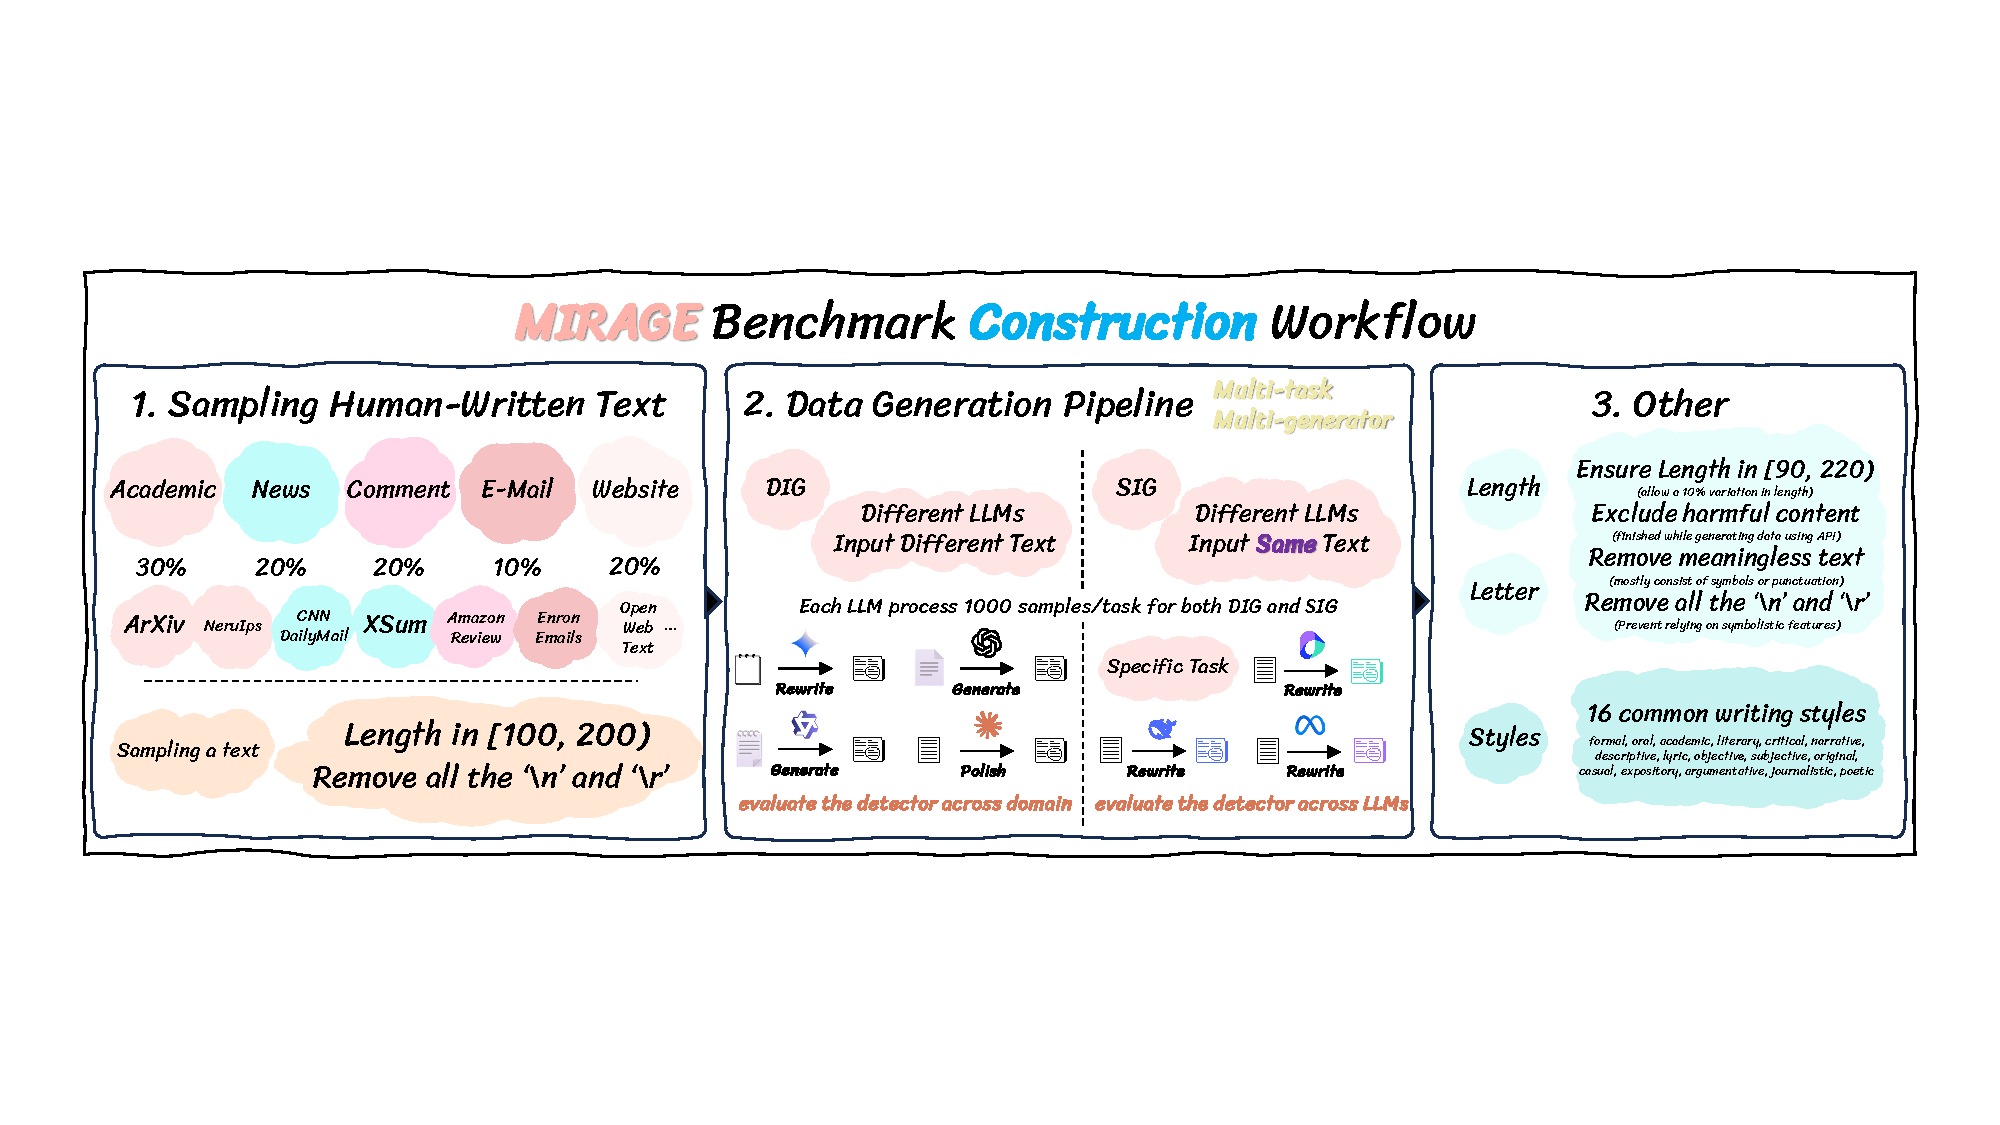
\includegraphics[width=\linewidth]{fig/workflow.pdf}
    \caption{The MIRAGE benchmark construction workflow. MIRAGE consists of 93K HWT-MGT pairs, significantly demonstrating diversity of text-domain, source LLM, and generation task, while using writing style control as augmentation. }
    \Description{Workflow of MIRAGE Benchmark.}
    \label{fig:workflow}
\end{figure*}